\documentclass[11pt,a4paper]{article}
\usepackage[utf8]{inputenc}
\usepackage{amsmath}
\usepackage{float}
\usepackage{amssymb}
\usepackage{graphicx}
\graphicspath{ {graphics/} }
    \title{Homework 03 - More Deterministic Finite Automata}
    \author{Gerardo Galván Olvera A01371872}
    \date{August 28 2017}
    \begin{document}
        \maketitle
                
        \begin{enumerate}
            \item The DFA \textbf{R1} accepts $\{\omega\mid\omega\text{begins with a 1 and ends with a 0}\}$:\\
                \begin{figure}[H]
                    \centering
                    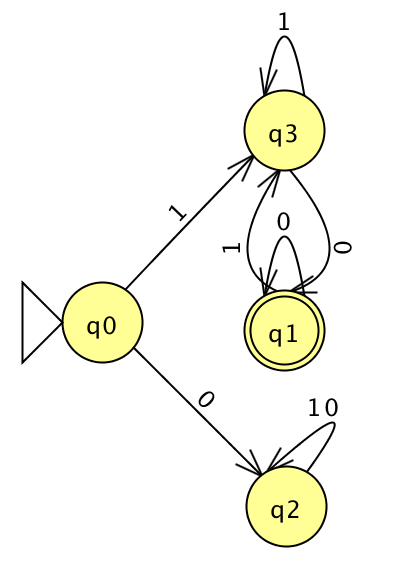
\includegraphics[width=0.50\textwidth]{A1}
                    \caption{The R1 DFA}
                \end{figure}

                For R1:
                \begin{enumerate}
                    \item $Q = \{q_0, q_1, q_2, q_3\}$
                    \item $\Sigma = \{0, 1\}$
                    \item $\delta \colon Q \times \Sigma \rightarrow Q =$
                    \begin{tabular}{c|c|c}
                         & 0 & 1 \\ \hline
                        $q_0$ & $q_2$ & $q_3$ \\ \hline
                        $q_1$ & $q_1$ & $q_3$ \\ \hline
                        $q_2$ & $q_2$ & $q_2$ \\ \hline
                        $q_3$ & $q_1$ & $q_3$ \\ \hline
                    \end{tabular}
                    \item $q_0$ (the start state) = $q_0 \in Q$
                    \item $F = \{q_1\}$
                \end{enumerate}

            \item The DFA \textbf{R2} accepts \[ \{\omega\mid\omega\text{ contains at least one 1 and an even number of 0s follow the last 1}\}\colon\]\\
                \begin{figure}[H]
                    \centering
                    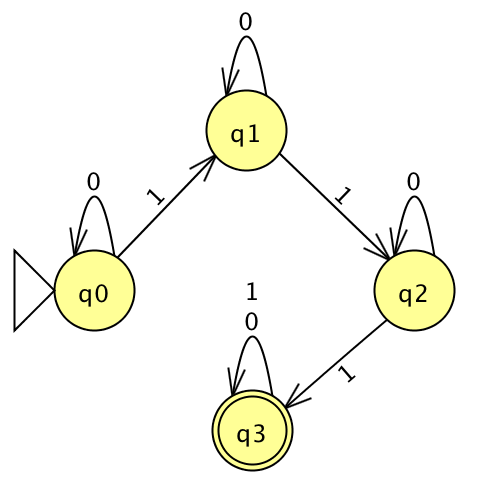
\includegraphics[width=0.50\textwidth]{A2}
                    \caption{The R2 DFA}
                \end{figure}

                For R2:
                \begin{enumerate}
                    \item $Q = \{q_0, q_1, q_2, q_3\}$
                    \item $\Sigma = \{0, 1\}$
                    \item $\delta \colon Q \times \Sigma \rightarrow Q =$
                    \begin{tabular}{c|c|c}
                         & 0 & 1 \\ \hline
                        $q_0$ & $q_0$ & $q_1$ \\ \hline
                        $q_1$ & $q_1$ & $q_2$ \\ \hline
                        $q_2$ & $q_2$ & $q_3$ \\ \hline
                        $q_3$ & $q_3$ & $q_3$ \\ \hline
                    \end{tabular}
                    \item $q_0$ (the start state) = $q_0 \in Q$
                    \item $F = \{q_3\}$
                \end{enumerate}

            \item The DFA \textbf{R3} accepts $\{\omega\mid\omega\text{ is the empty string $\epsilon$ or ends in a 0}\}$:

                \begin{figure}[H]
                    \centering
                    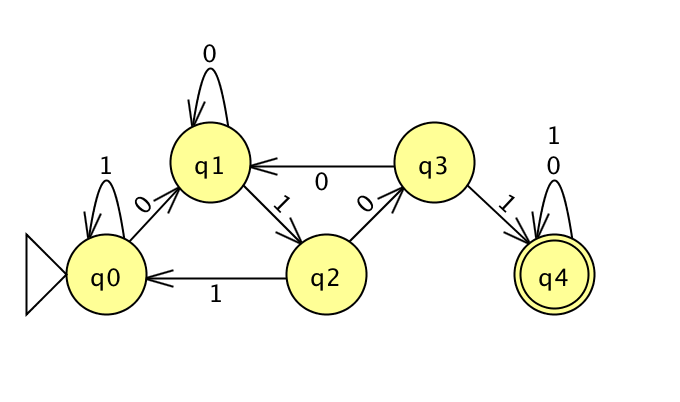
\includegraphics[width=0.50\textwidth]{A3}
                    \caption{The R3 DFA}
                \end{figure}

                For R3:
                \begin{enumerate}
                    \item $Q = \{q_0, q_1, q_2, q_3, q_4\}$
                    \item $\Sigma = \{0, 1\}$
                    \item $\delta \colon Q \times \Sigma \rightarrow Q =$
                    \begin{tabular}{c|c|c}
                         & 0 & 1 \\ \hline
                        $q_0$ & $q_1$ & $q_0$ \\ \hline
                        $q_1$ & $q_1$ & $q_2$ \\ \hline
                        $q_2$ & $q_3$ & $q_0$ \\ \hline
                        $q_3$ & $q_1$ & $q_4$ \\ \hline
                        $q_4$ & $q_4$ & $q_4$ \\ \hline
                    \end{tabular}
                    \item $q_0$ (the start state) = $q_0 \in Q$
                    \item $F = \{q_4\}$
                \end{enumerate}

            \item The DFA \textbf{R4} accepts $\{\omega\mid\omega\text{ contains at least one 1 and ends with 1}\}$:
                \begin{figure}[H]
                    \centering
                    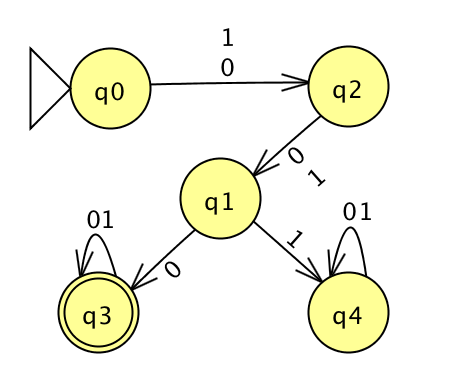
\includegraphics[width=0.50\textwidth]{A4}
                    \caption{The R4 DFA}
                \end{figure}

                For R4:
                \begin{enumerate}
                    \item $Q = \{q_0, q_1, q_2, q_3, q_4\}$
                    \item $\Sigma = \{0, 1\}$
                    \item $\delta \colon Q \times \Sigma \rightarrow Q =$
                    \begin{tabular}{c|c|c}
                         & 0 & 1 \\ \hline
                        $q0$ & $q2$ & $q2$ \\ \hline
                        $q1$ & $q3$ & $q4$ \\ \hline
                        $q2$ & $q1$ & $q1$ \\ \hline
                        $q3$ & $q3$ & $q3$ \\ \hline
                        $q4$ & $q4$ & $q4$ \\ \hline
                    \end{tabular}
                    \item $q_0$ (the start state) = $q_0 \in Q$
                    \item $F = \{q_3\}$
                \end{enumerate}

            \item The DFA \textbf{R5} accepts $\{\omega\mid\omega\text{ starts and ends with the same symbol}\}$:\\
                \begin{figure}[H]
                    \centering
                    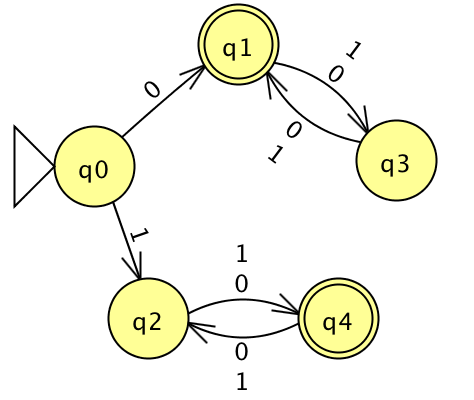
\includegraphics[width=0.50\textwidth]{A5}
                    \caption{The R5 DFA}
                \end{figure}

                For R5:
                \begin{enumerate}
                    \item $Q = \{q_0, q_1, q_2, q_3, q_4\}$
                    \item $\Sigma = \{0, 1\}$
                    \item $\delta \colon Q \times \Sigma \rightarrow Q =$
                    \begin{tabular}{c|c|c}
                         & 0 & 1 \\ \hline
                        $q_0$ & $q_1$ & $q_2$ \\ \hline
                        $q_1$ & $q_3$ & $q_3$ \\ \hline
                        $q_2$ & $q_4$ & $q_4$ \\ \hline
                        $q_3$ & $q_1$ & $q_1$ \\ \hline
                        $q_4$ & $q_2$ & $q_2$ \\ \hline
                    \end{tabular}
                    \item $q_0$ (the start state) = $q_0 \in Q$
                    \item $F = \{q_1, q_4\}$
                \end{enumerate}

            \item The DFA \textbf{R6} accepts $\{\omega\mid\omega\text{contains a substring 001}\}$:\\
                \begin{figure}[H]
                    \centering
                    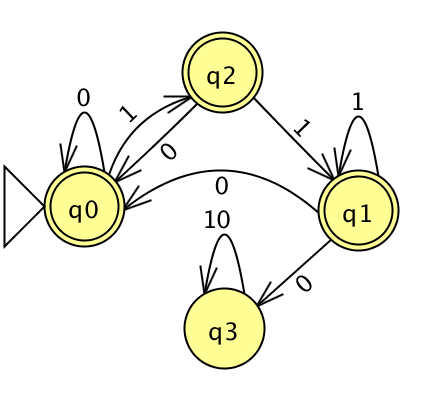
\includegraphics[width=0.50\textwidth]{A6}
                    \caption{The R6 DFA}
                \end{figure}

                For R6:
                \begin{enumerate}
                    \item $Q = \{q_0, q_1, q_2, q_3\}$
                    \item $\Sigma = \{0, 1\}$
                    \item $\delta \colon Q \times \Sigma \rightarrow Q =$
                    \begin{tabular}{c|c|c}
                         & 0 & 1 \\ \hline
                        $q_0$ & $q_0$ & $q_2$ \\ \hline
                        $q_1$ & $q_0$ & $q_1$ \\ \hline
                        $q_2$ & $q_0$ & $q_1$ \\ \hline
                        $q_3$ & $q_3$ & $q_3$ \\ \hline
                    \end{tabular}
                    \item $q_0$ (the start state) = $q_0 \in Q$
                    \item $F = \{q_0, q_1, q_2\}$
                \end{enumerate}

            \item The DFA \textbf{R7} accepts tuples of the form (front door switch state, rear door switch state):\\
            \begin{figure}[H]
                \centering
                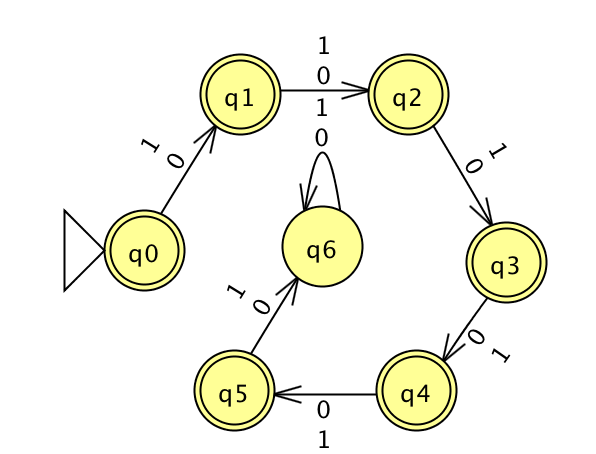
\includegraphics[width=0.75\textwidth]{A7}
                \caption{The R6 DFA}
            \end{figure}

            For R7:
            \begin{enumerate}
                \item $Q = \{q_0, q_1, q_2, q_3, q_4, q_5, q_6\}$
                \item $\Sigma = \{0, 1\}$
                \item $\delta \colon Q \times \Sigma \rightarrow Q =$
                \begin{tabular}{c|c|c}
                     & 0 & 1 \\ \hline
                    $q_0$ & $q_1$ & $q_1$ \\ \hline
                    $q_1$ & $q_2$ & $q_2$ \\ \hline
                    $q_2$ & $q_3$ & $q_3$ \\ \hline
                    $q_3$ & $q_4$ & $q_4$ \\ \hline
                    $q_4$ & $q_5$ & $q_5$ \\ \hline
                    $q_5$ & $q_6$ & $q_6$ \\ \hline
                    $q_6$ & $q_6$ & $q_6$ \\ \hline
                \end{tabular}
                \item $q_0$ (the start state) = $q_0 \in Q$
                \item $F = \{q_0, q_1, q_2, q_3, q_4, q_5\}$
            \end{enumerate}


            
            
        \end{enumerate}
            
        % \begin{thebibliography}
        %     \bibitem{} Graham, R. L. (1994). Concrete mathematics: a foundation for computer science. Pearson Education India.
        % \end{thebibliography}

    \end{document}
